\documentclass{beamer}
\usepackage[utf8]{inputenc}
\usepackage{caption}
\usepackage{subcaption}
\usepackage{tabularx}

\newenvironment{changemargin}[2]{%
  \begin{list}{}{%
    \setlength{\topsep}{0pt}%
    \setlength{\leftmargin}{#1}%
    \setlength{\rightmargin}{#2}%
    \setlength{\listparindent}{\parindent}%
    \setlength{\itemindent}{\parindent}%
    \setlength{\parsep}{\parskip}%
  }%
  \item[]}{\end{list}}

\usetheme{Darmstadt}

\title{Animat}
\subtitle{Using coloured snapshots for short-range guidance in mobile robots}
\author{Paul Moncuquet \& Thibaut Munzer}

\begin{document}

\begin{frame}
  \titlepage
\end{frame}

\begin{frame}
  \frametitle{Sommaire}
  \tableofcontents%[pausesections]
\end{frame}

\section{Introduction}

\subsection{Problématique}

\begin{frame}
  \frametitle{Problématique}
  \begin{block}{\textit{Homming}}
  \begin{itemize}
    \item Snapsot du goal
    \item Près du goal
    \item Utilisation de données visuelle
    \item Methode basé sur le matching d'amer    
  \end{itemize}
  \end{block}

  \begin{block}{\textit{Approche Animat}}
  \begin{itemize}
    \item Transposition du comportement des abeilles dans un contexte robotique
    \item angle de vue 220
    \item Par exemple retour a la base d'alimentation
  \end{itemize}
  \end{block}
\end{frame}

\subsection{Travaux existant}

\begin{frame}
  \title{Cartwright \& Collett}
  \begin{block}{Cartwright \& Collett}
    \begin{itemize}
      \item Inspiré des abeille
      \item Hypothèse : orientation connue
      \item Création d'un pannoramma
      \item Matching au plus proche
      \item Calcul des composantes tangentielles et radiales    
      \begin{figure}
        \centering
        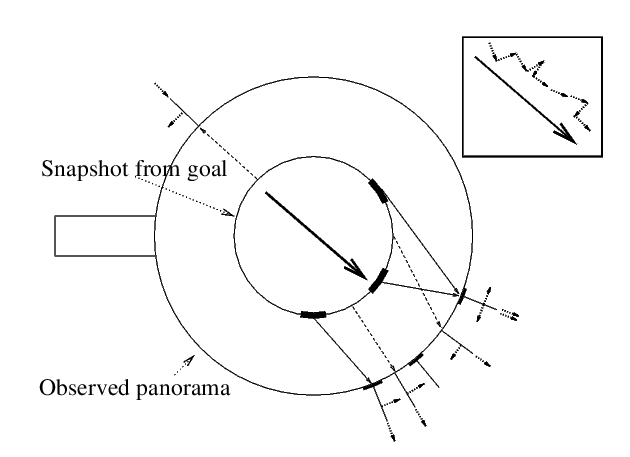
\includegraphics[scale=0.2]{cc_model.png}
        \caption{CC Modèle}
      \end{figure}
    \end{itemize}
  \end{block}
\end{frame}

\begin{frame}
  \begin{block}{PV Modèle}
    \begin{itemize}
      \item Proposé par Möller et al. \cite{TODO}
      \item Contribution de chaque vecteur proportionelle à la différence lors du matching
    \end{itemize}
  \end{block}
  \begin{block}{Gourichon Modèle}
    \begin{itemize}
      \item modèle de l'article étudié
      \item Basé sur le PV modèle
      \item Hypothèse d'orientation fixe
      \item Amélioration du matching
      \item Utilisation de la couleur 
      \item suppression de la composante radial
    \end{itemize}
  \end{block}
\end{frame}

\section{Matériels, méthodes et résultats}


\begin{frame}
  Deux expériences dans l'article :
  \begin{itemize}
    \item Une expérience virtuelle
    \begin{figure}
      \centering
      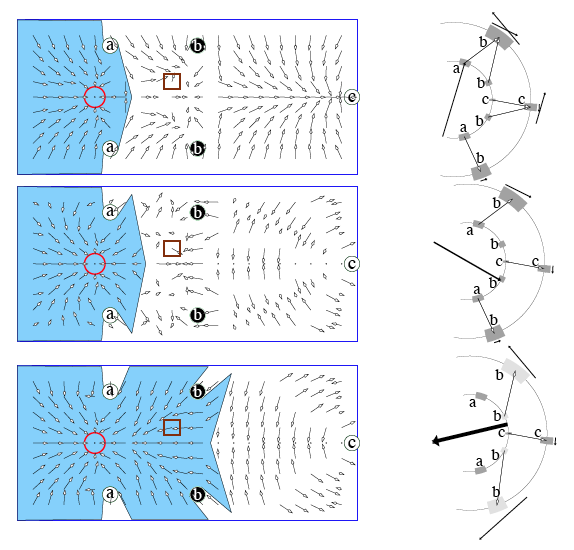
\includegraphics[scale=0.2]{Exp-virtuel.png}
    \end{figure}
    \item Une expérience réelle
    \begin{figure}
      \centering
      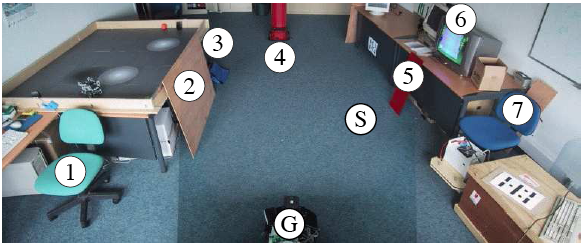
\includegraphics[scale=0.2]{Exp-real.png}
    \end{figure}
  \end{itemize}
  Reproduction de l'éxpérience virtuelle

\end{frame}

\subsection{Reproduction des résultats}

\begin{frame}
  \begin{block}{Mise en place d'un simulateur}
    \begin{itemize}
      \item Choix de ne pas utiliser un simulateur existant
      \item Utilisation de SDL
    \end{itemize}
  \end{block}
  \begin{figure}
    \centering
    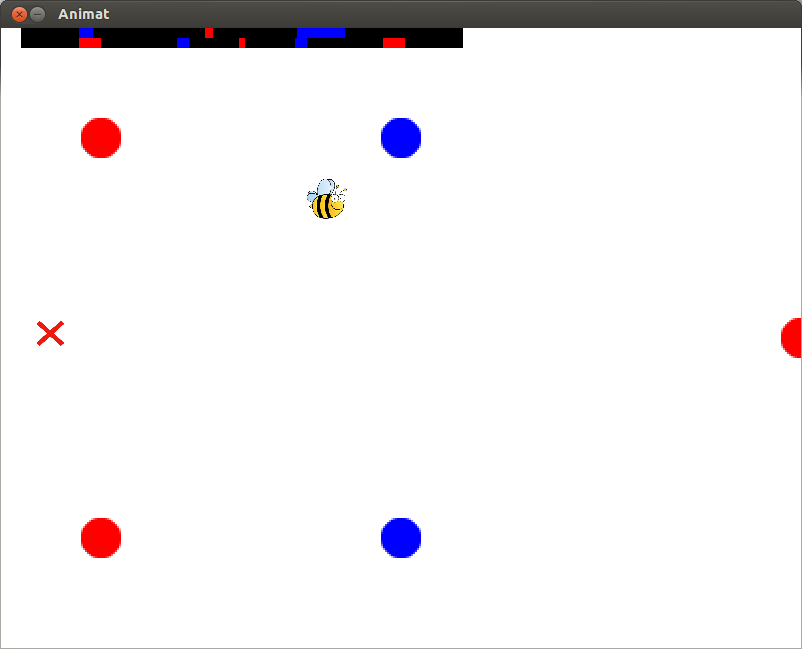
\includegraphics[scale=0.2]{one_run.png}
    \caption{Exemple simulateur}
  \end{figure}
\end{frame}

\begin{frame}
  \begin{block}{Calcul de la zone de convergence}
    \begin{itemize}
      \item Discrétization du monde
      \item Problème du cas d'arret
      \item Optimization du calcul
    \end{itemize}
  \end{block}
  \begin{figure}
    \centering
    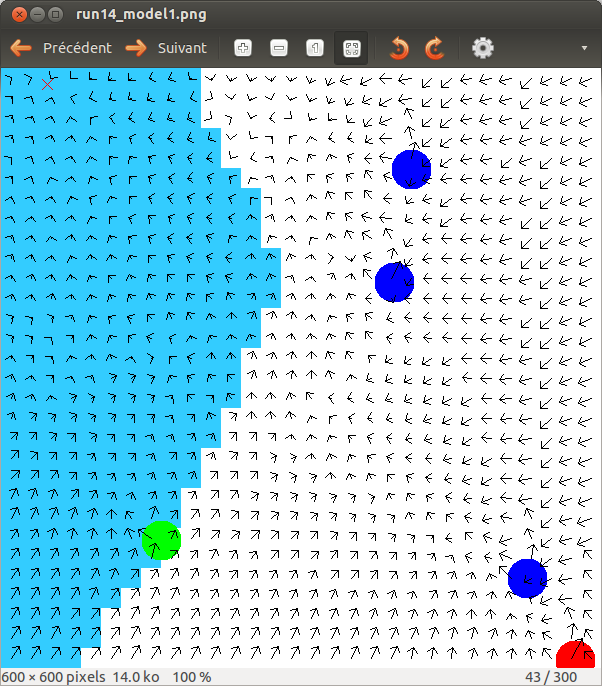
\includegraphics[scale=0.2]{exp.png}
    \caption{Exemple zone de convergence}
  \end{figure}
\end{frame}

\subsection{Comparaison des résultat}

\begin{frame}
  \frametitle{PV modèle}
  \begin{figure}
    \centering
    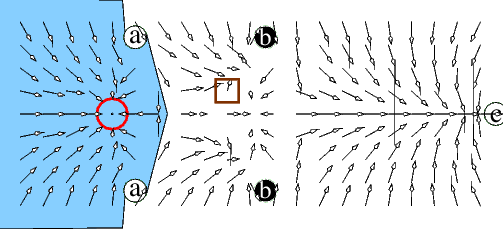
\includegraphics[scale=0.3]{pv_article.png}
  \end{figure}
  \begin{figure}
    \centering
    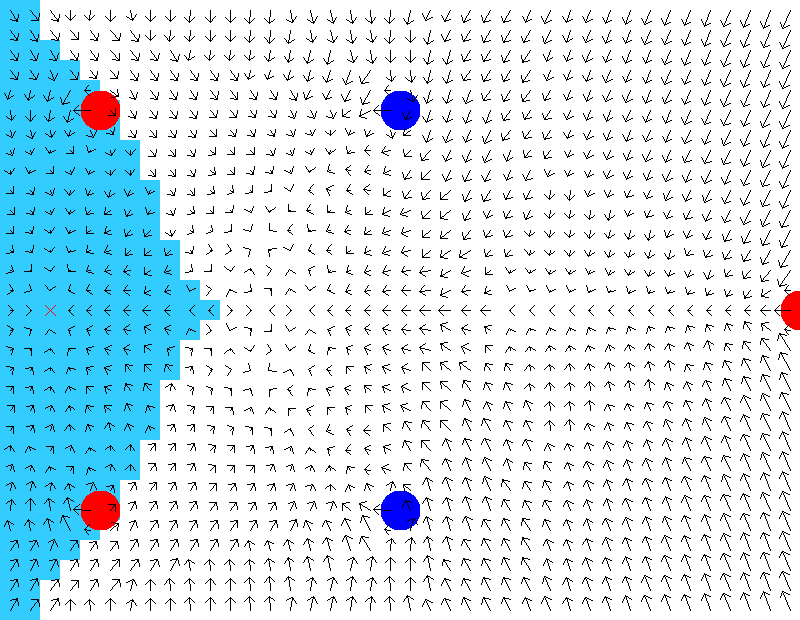
\includegraphics[scale=0.15]{pv1_res.png}
    \caption{Comparaison PV modèle}
  \end{figure}  
\end{frame}

\begin{frame}
  \frametitle{PV modèle : Contributions modifiées}
  \begin{figure}
    \centering
    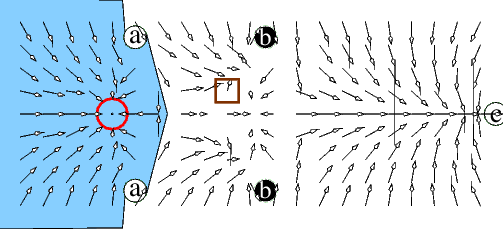
\includegraphics[scale=0.3]{pv_article.png}
  \end{figure}
  \begin{figure}
    \centering
    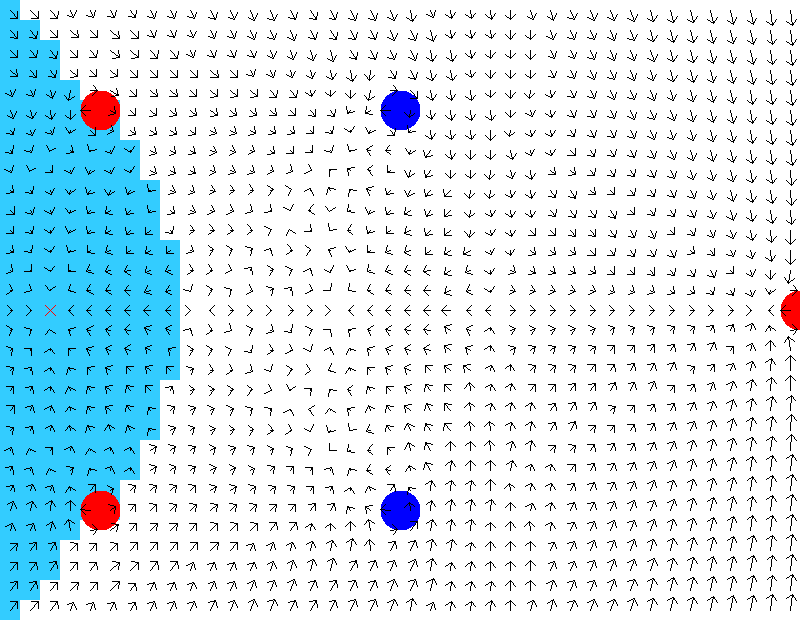
\includegraphics[scale=0.15]{pv2_res.png}
    \caption{Comparaison PV modèle}
  \end{figure}  
\end{frame}

\begin{frame}
  \frametitle{Gournichon modèle sans couleur}
  \begin{figure}
    \centering
    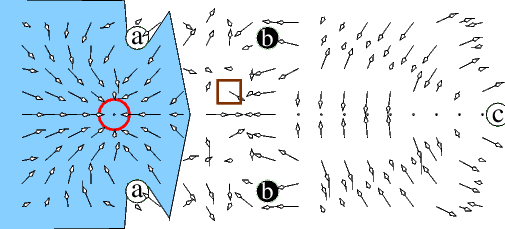
\includegraphics[scale=0.3]{nocolor_article.png}
  \end{figure}
  \begin{figure}
    \centering
    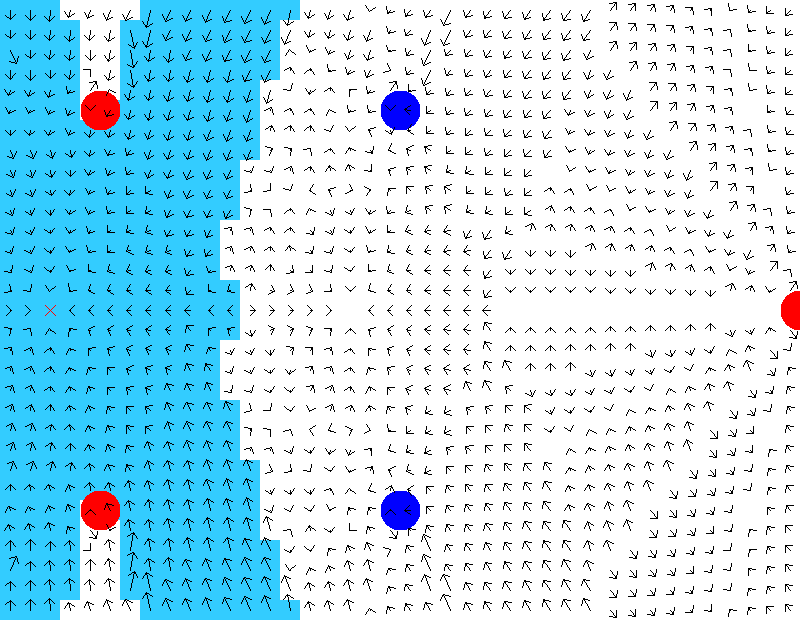
\includegraphics[scale=0.15]{nocolor_res.png}
    \caption{Comparaison Gournichon modèle sans couleur}
  \end{figure}  
\end{frame}

\begin{frame}
  \frametitle{Gournichon modèle}
  \begin{figure}
    \centering
    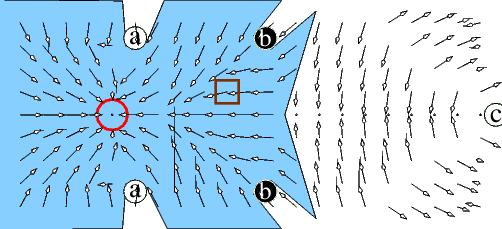
\includegraphics[scale=0.3]{color_article.png}
  \end{figure}
  \begin{figure}
    \centering
    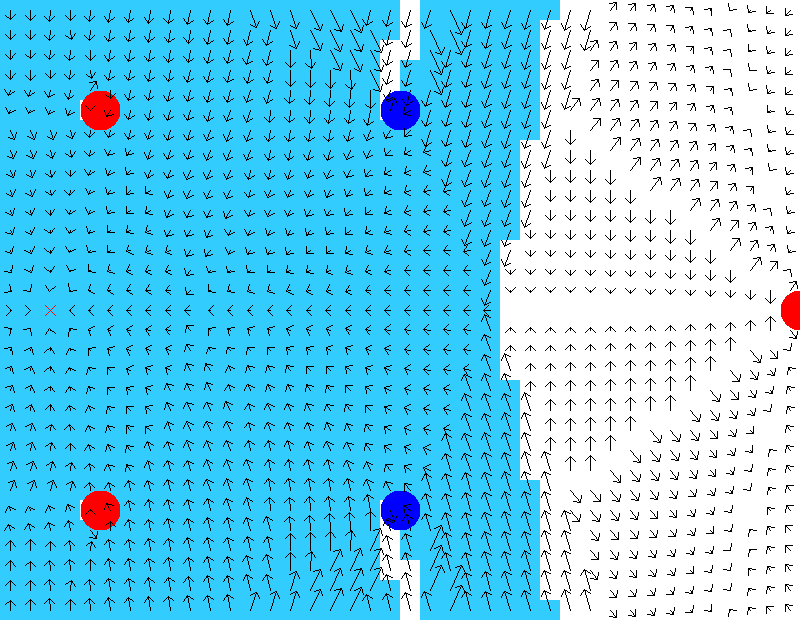
\includegraphics[scale=0.15]{color_res.png}
    \caption{Comparaison Gournichon modèle}
  \end{figure}  
\end{frame}

\section{Discussion et conclusion}

\subsection{Discussion}

\begin{frame}
  \frametitle{Etude des performances sur un grand nombre de scène}
  \begin{changemargin}{-1.0cm}{0cm}
  \begin{figure}
    \centering
    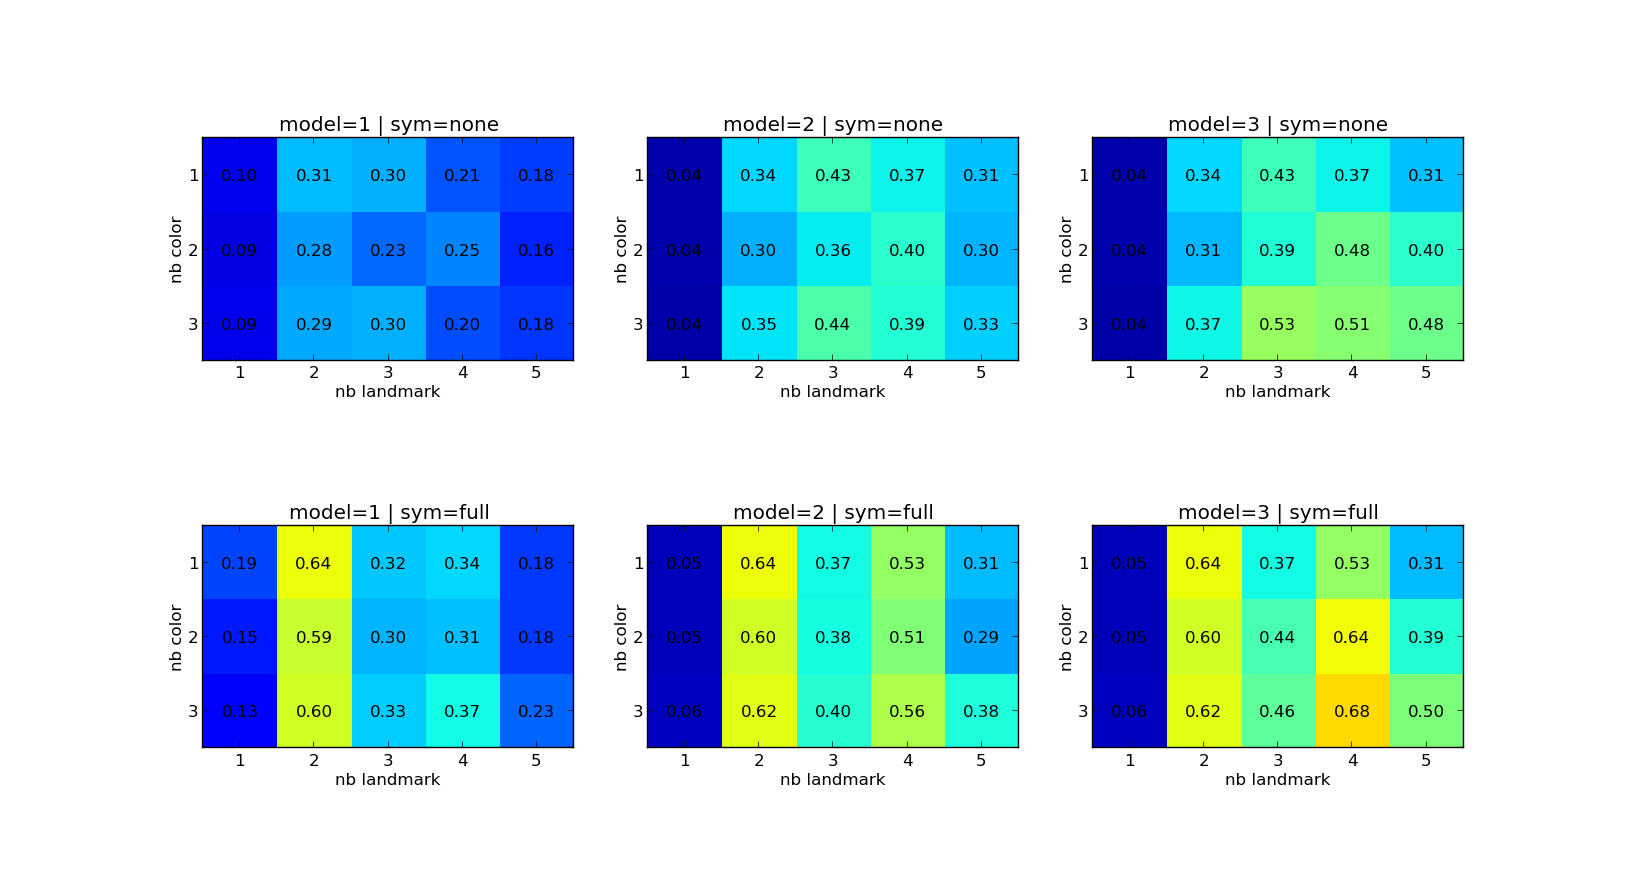
\includegraphics[scale=0.3]{res_sym.png}
  \end{figure}  
  \end{changemargin}
\end{frame}

\begin{frame}
  \frametitle{Etude des performances sur un grand nombre de scène}
  \begin{changemargin}{-1.0cm}{0cm}
  \begin{figure}
    \centering
    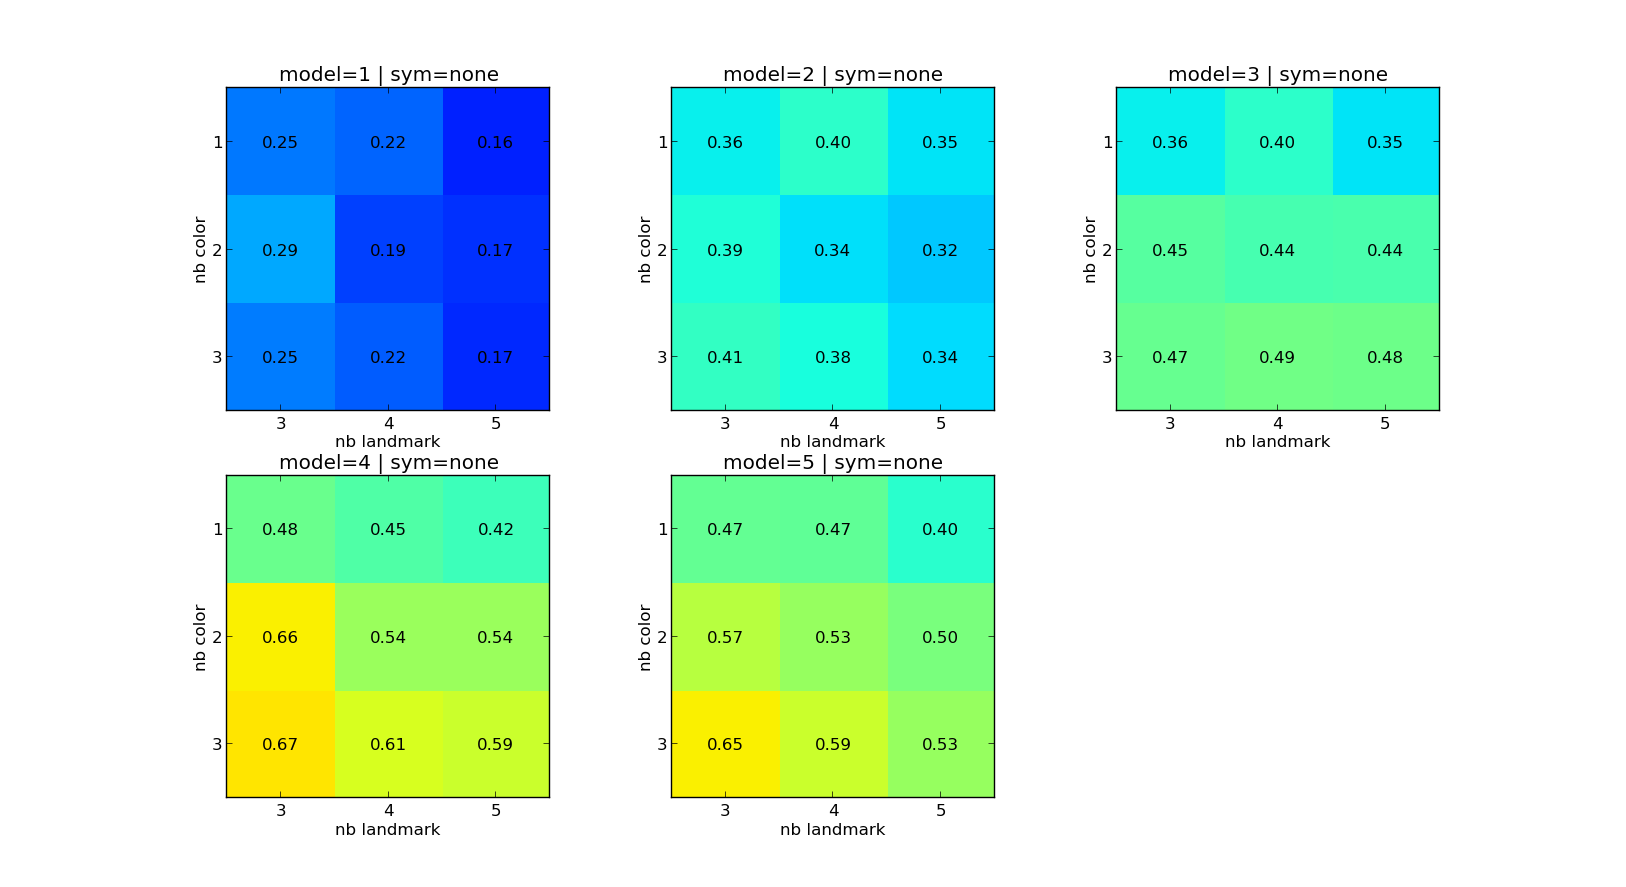
\includegraphics[scale=0.3]{res_45.png}
  \end{figure}  
  \end{changemargin}
\end{frame}

\subsection{Conclusion}% Conclusion

\begin{frame}
  \frametitle{Conclusion}
  \begin{itemize}
    \item Lecture et compréhension d'un article
    \item Reproduction des résultats
    \item Amélioration du processus de validation du modèle proposé
    \item Réintégration de la composante radial et amélioration des résultats    
  \end{itemize}
\end{frame}

\end{document}